\clearpage
\myparagraph{\RU{Первый пример с \olly}\EN{First \olly example}: a=1.2 \AndENRU b=3.4}
\index{\olly}

\RU{Загружаем пример в}\EN{Let's load the example into} \olly:

\begin{figure}[H]
\centering
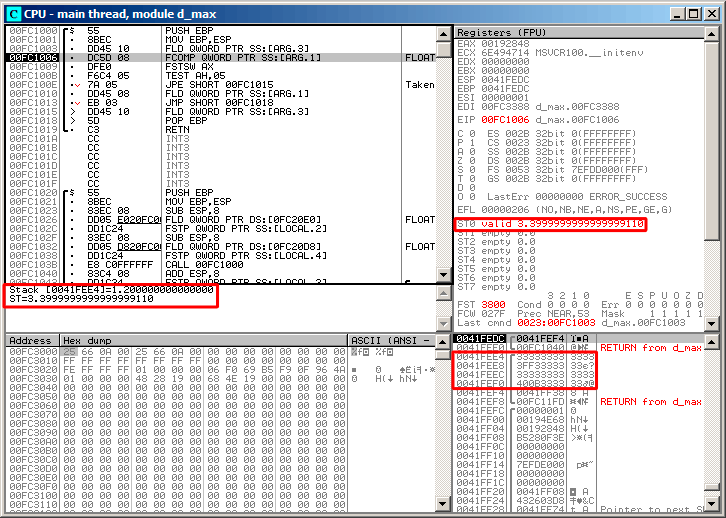
\includegraphics[scale=\FigScale]{patterns/12_FPU/3_comparison/x86/MSVC/olly1_1.png}
\caption{\olly: \RU{первая \FLD исполнилась}\EN{first \FLD is executed}}
\label{fig:FPU_comparison_case1_olly1}
\end{figure}

\RU{Текущие параметры функции}\EN{Current arguments of the function}: $a=1.2$ \AndENRU $b=3.4$ 
(\RU{их видно в стеке: 2 пары 32-битных значений}\EN{We can see them in the stack: two pairs of 32-bit values}).
$b$ ($3.4$) \RU{уже загружено в}\EN{is already loaded in} \ST{0}.
\RU{Сейчас будет исполняться \FCOMP}\EN{Now \FCOMP is being executed}. 
\olly \RU{показывает второй аргумент для \FCOMP, который сейчас находится в стеке}\EN{shows the second \FCOMP
argument, which is in stack right now}.

\clearpage
\FCOMP \RU{отработал}\EN{is executed}:

\begin{figure}[H]
\centering
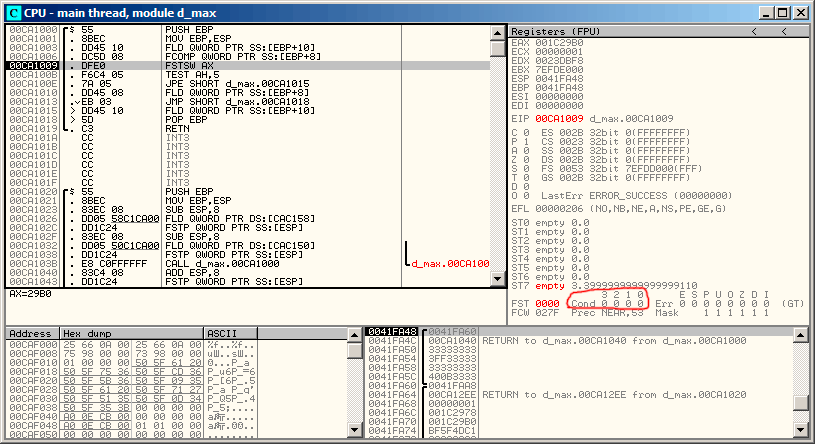
\includegraphics[scale=\FigScale]{patterns/12_FPU/3_comparison/x86/MSVC/olly1_2.png}
\caption{\olly: \FCOMP \RU{исполнилась}\EN{is executed}}
\label{fig:FPU_comparison_case1_olly2}
\end{figure}

\RU{Мы видим состояния condition-флагов \ac{FPU}}\EN{We see the state of the \ac{FPU}'s condition flags}: 
\RU{все нули}\EN{all zeroes}.
\RU{Вытолкнутое значение отображается как \ST{7}, почему это так, я писал раннее}
\EN{The popped value is reflected as \ST{7}, I wrote earlier about reason for this}: 
\myref{FPU_is_rather_circular_buffer}.

\clearpage
\FNSTSW \RU{сработал}\EN{is executed}:
\begin{figure}[H]
\centering
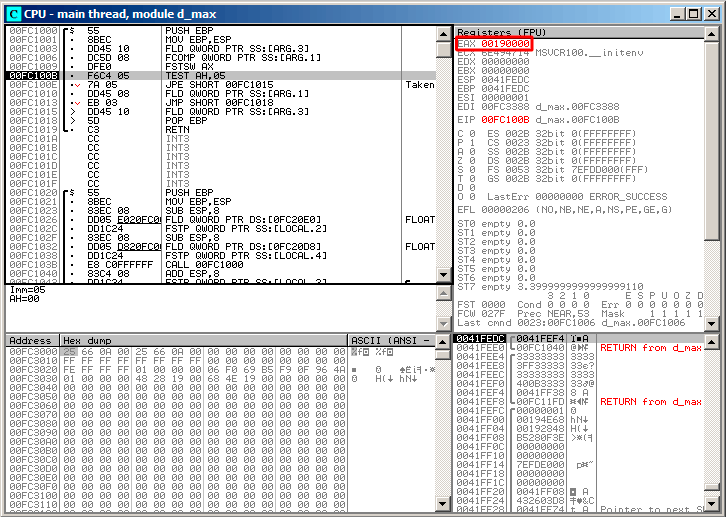
\includegraphics[scale=\FigScale]{patterns/12_FPU/3_comparison/x86/MSVC/olly1_3.png}
\caption{\olly: \FNSTSW \RU{исполнилась}\EN{is executed}}
\label{fig:FPU_comparison_case1_olly3}
\end{figure}

\RU{Видно, что регистр \TT{AX} содержит нули: действительно, ведь все condition-флаги тоже содержали нули.}
\EN{We see that the \TT{AX} register contain zeroes: indeed, all condition flags are zero.}
(\olly \RU{дизассемблирует команду}\EN{disassembles the} \FNSTSW \RU{как}\EN{instruction as} \TT{FSTSW} --- 
\RU{это синоним}\EN{they are synonyms}).

\clearpage
\TEST \RU{сработал}\EN{is executed}:

\begin{figure}[H]
\centering
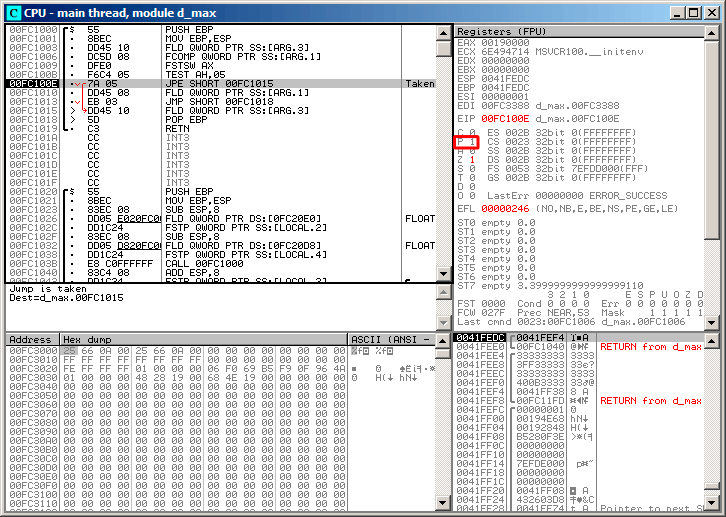
\includegraphics[scale=\FigScale]{patterns/12_FPU/3_comparison/x86/MSVC/olly1_4.png}
\caption{\olly: \TEST \RU{исполнилась}\EN{is executed}}
\label{fig:FPU_comparison_case1_olly4}
\end{figure}

\RU{Флаг \TT{PF} равен единице.}\EN{The \TT{PF} flag is set to $1$.}
\RU{Все верно: количество выставленных бит в $0$ --- это $0$, а $0$ --- это четное число.}
\EN{Indeed: the number of bits set in $0$ is $0$ and $0$ is an even number.}
\olly \RU{дизассемблирует}\EN{disassembles} \TT{JP} \RU{как}\EN{as} \ac{JPE} --- \RU{это синонимы}\EN{they
are synonyms}.
\RU{И она сейчас сработает}\EN{And it is about to trigger now}.

\clearpage
\ac{JPE} \RU{сработала}\EN{triggered}, \FLD \RU{загрузила в \ST{0} значение $b$ ($3.4$)}
\EN{loads the value of $b$ ($3.4$) in \ST{0}}:

\begin{figure}[H]
\centering
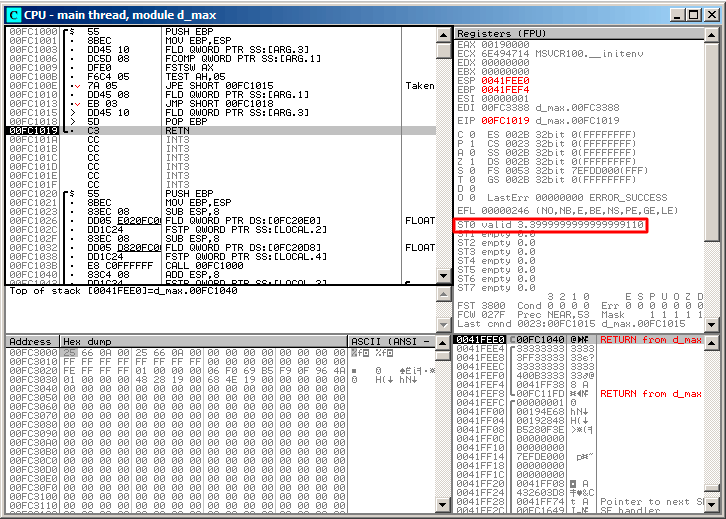
\includegraphics[scale=\FigScale]{patterns/12_FPU/3_comparison/x86/MSVC/olly1_5.png}
\caption{\olly: \RU{вторая \FLD исполнилась}\EN{second \FLD is executed}}
\label{fig:FPU_comparison_case1_olly5}
\end{figure}

\RU{Ф-ция заканчивает свою работу}\EN{The function finishes its work}.

\clearpage
\myparagraph{\RU{Второй пример с \olly}\EN{Second \olly example}: a=5.6 \AndENRU b=-4}

\RU{Загружаем пример в}\EN{Let's load example into} \olly:

\begin{figure}[H]
\centering
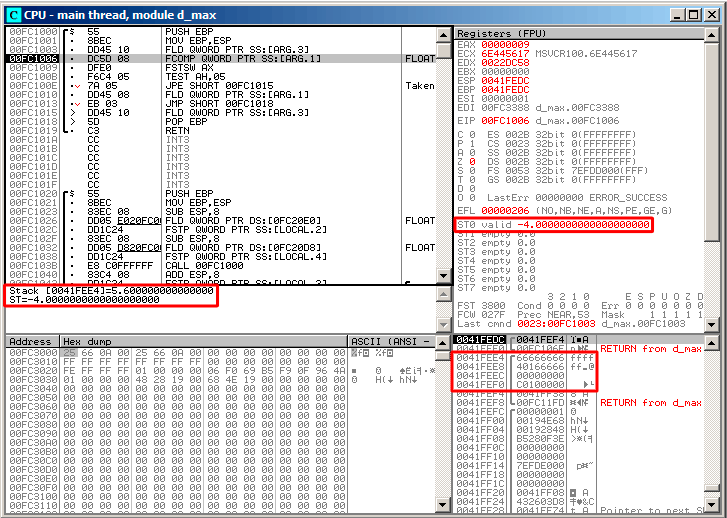
\includegraphics[scale=\FigScale]{patterns/12_FPU/3_comparison/x86/MSVC/olly2_1.png}
\caption{\olly: \RU{первая \FLD исполнилась}\EN{first \FLD executed}}
\label{fig:FPU_comparison_case2_olly1}
\end{figure}

\RU{Текущие параметры функции}\EN{Current function arguments}: $a=5.6$ \AndENRU $b=-4$).
$b$ ($-4$) \RU{уже загружено в}\EN{is already loaded in} \ST{0}.
\RU{Сейчас будет исполняться \FCOMP}\EN{\FCOMP about to execute now}. 
\olly \RU{показывает второй аргумент \FCOMP, который сейчас находится в стеке}
\EN{shows the second \FCOMP argument, which is in stack right now}.

\clearpage
\FCOMP \RU{отработал}\EN{executed}:

\begin{figure}[H]
\centering
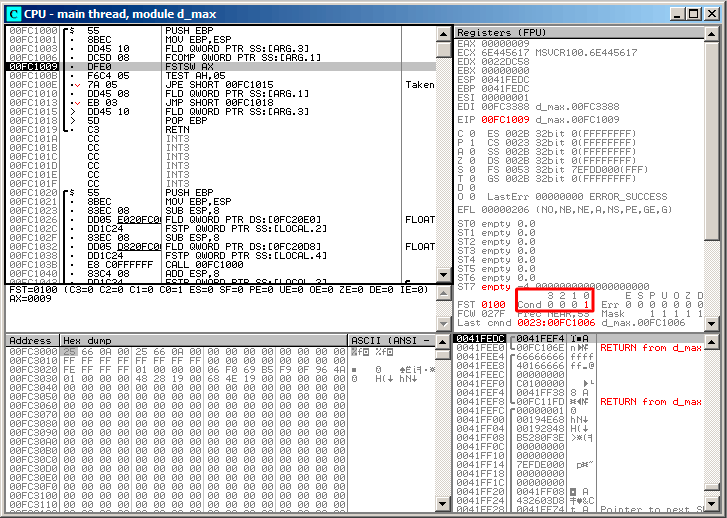
\includegraphics[scale=\FigScale]{patterns/12_FPU/3_comparison/x86/MSVC/olly2_2.png}
\caption{\olly: \FCOMP \RU{исполнилась}\EN{executed}}
\label{fig:FPU_comparison_case2_olly2}
\end{figure}

\RU{Мы видим значения condition-флагов \ac{FPU}: все нули кроме \Czero.}
\EN{We see the state of the \ac{FPU}'s condition flags: all zeroes except \Czero.}

\clearpage
\FNSTSW \RU{сработал}\EN{executed}:

\begin{figure}[H]
\centering
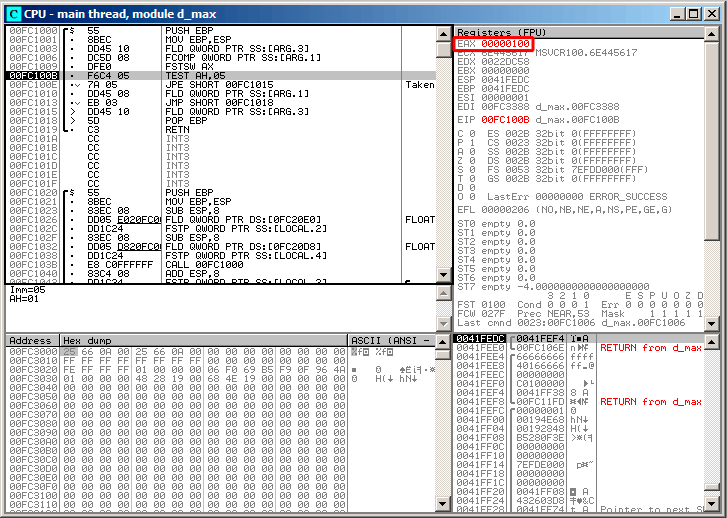
\includegraphics[scale=\FigScale]{patterns/12_FPU/3_comparison/x86/MSVC/olly2_3.png}
\caption{\olly: \FNSTSW \RU{исполнилась}\EN{executed}}
\label{fig:FPU_comparison_case2_olly3}
\end{figure}

\RU{Видно, что регистр \TT{AX} содержит \TT{0x100}: флаг \Czero стал на место 16-го бита.}
\EN{We see that the \TT{AX} register contains \TT{0x100}: the \Czero flag is at the 16th bit.}

\clearpage
\TEST \RU{сработал}\EN{executed}:

\begin{figure}[H]
\centering
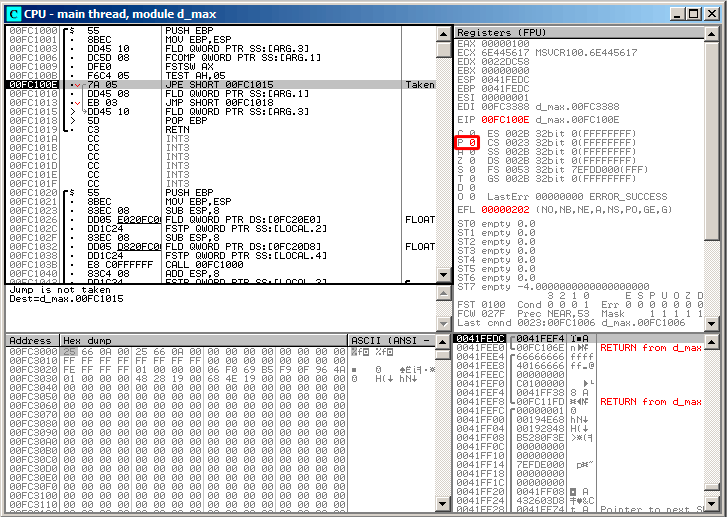
\includegraphics[scale=\FigScale]{patterns/12_FPU/3_comparison/x86/MSVC/olly2_4.png}
\caption{\olly: \TEST \RU{исполнилась}\EN{executed}}
\label{fig:FPU_comparison_case2_olly4}
\end{figure}

\EN{The}\RU{Флаг} \TT{PF} \RU{равен нулю}\EN{ flag is cleared}.
\RU{Все верно}\EN{Indeed}: 
\RU{количество единичных бит в \TT{0x100} --- это $1$, а $1$ --- это нечетное число}
\EN{the count of bits set in \TT{0x100} is $1$ and $1$ is an odd number}.
\ac{JPE} \RU{сейчас не сработает}\EN{is being skipped now}.

\clearpage
\ac{JPE} \RU{не сработала, }\EN{wasn't triggered, so} \FLD 
\RU{загрузила в \ST{0} значение $a$ ($5.6$)}
\EN{loads the value of $a$ ($5.6$) in \ST{0}}:

\begin{figure}[H]
\centering
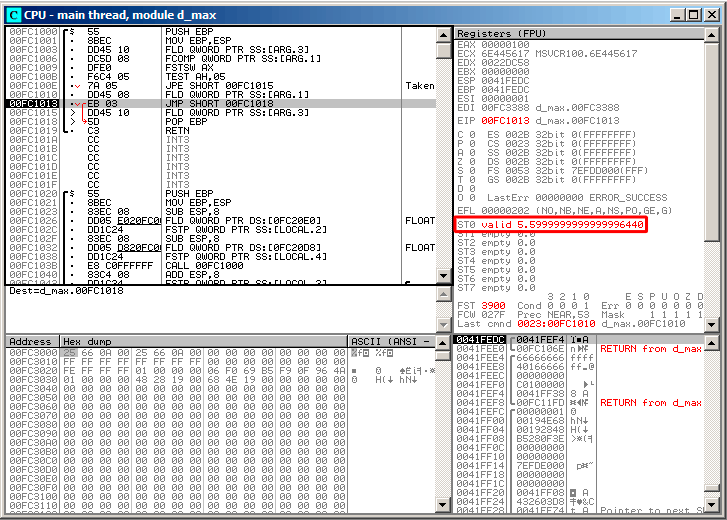
\includegraphics[scale=\FigScale]{patterns/12_FPU/3_comparison/x86/MSVC/olly2_5.png}
\caption{\olly: \RU{вторая \FLD исполнилась}\EN{second \FLD executed}}
\label{fig:FPU_comparison_case2_olly5}
\end{figure}

\RU{Ф-ция заканчивает свою работу}\EN{The function finishes its work}.
